\section{Results}
\label{sec:results}

Following the methodology described in the previous section, we estimate the total U.S. Resource to be 3300 TWh/yr, and up to 4090 TWh/yr when including the potential resource (Table~\ref{table:totals}). This is an increase of  25\% compared to earlier DOE wave resource assessments. This result, however, should not be interpreted as an indication of a growing resource (e.g., due to climate change). Instead, the increase is due simply to a more complete accounting of wave energy sources (i.e., the ``local resource''), and from extending the domain to include the vast U.S. EEZ. In other words, while the local resource is a sizable and valid piece of the total \textit{theoretical} resource, it is likely to be especially technically challenging to harness.

\subsection{Refined estimates by region}

Nearly two-thirds of the nation's wave energy resource is in Alaska where a large resource area and energetic waves in the North Pacific combine to create a large total (2000 – 2550 TWh/yr).

The U.S. West Coast has a large remote resource (420 TWh/yr) where energetic waves from the Pacific arrive from offshore.  The West Coast local resource is relatively modest in comparison (90 - 210 TWh/yr).

The U.S. East Coast resource, on the other hand, is composed primarily of the local resource (180 – 230 TWh/yr) and has a relatively modest remote piece (110 TWh/yr). This is because mid-latitude westerly winds tend to generate wave energy that propagates eastward and builds to a sizable resource across the broad fetch of the U.S. EEZ. Relatively less wave energy from the open ocean propagates onshore toward the U.S. eastern coastline (compared to the U.S. west coast).

Hawaii has a large resource due largely to waves that arrive from the North Pacific along the northern boundary of the EEZ. The natural local resource is relatively small, due primarily to the fact that the sea-state in this region is -- in the long-average perspective presented here -- roughly `steady-state' because the wind input and dissipation are approximately in balance.

The Gulf of Mexico and Caribbean regions have a modest wave resource composed predominantly of local wind input. The remote resource in this region is very small because the majority of the U.S. EEZ boundary throughout this region borders other EEZs (\ref{appendix:one-way-method}).

\subsection{The Inner Shelf Resource}

In order to identify a more realistic near-term estimate of the wave resource (e.g., for the next decade or so) we also compute $R_T$ using a 10 nautical-mile boundary, and refer to this as the ``inner shelf'' resource (last column in Table \ref{table:totals}). In this case, the local resource (both $R_{L_\circ}$ and $R_{L_*}$) is small for all regions (5\% in Alaska, <2\% for all other regions), so we have only presented $R_T$.

The inner-shelf resource totals are somewhat surprising because even though they are composed primarily of the remote resource several regions (Alaska, the Gulf of Mexico, as well as Puerto Rico and the U.S. Virgin Islands) actually have a larger inner-shelf resource than remote resource at the EEZ. This is mostly due to the fact that the inner-shelf integration contour is actually {\em longer} than the EEZ contour in these regions. This, in turn, is partly due to the geometry of the region (e.g., the Gulf of Mexico), and also to the fact that the EEZ contour does not include borders with other nation's EEZs while the `inner shelf' resource is not clipped in this way (e.g., Puerto Rico). The energy input by the wind between 200 and 10 nautical-miles from shore may also play a role. 

It is also interesting that the west coast inner-shelf resource (95.5\% remote) is very nearly the same as the resource at the edge of the EEZ. This suggests that the vast majority of the wave energy generated by local winds between the EEZ and the inner-shelf contour actually propagates offshore.

The Hawaiian resource decreases significantly from the EEZ to inner-shelf because the latter -- i.e., the 10 nautical-mile boundary, which is actually four separate contours around island groups -- is much shorter than the full EEZ boundary. The east coast inner-shelf resource is somewhat smaller than the EEZ remote resource because some of that energy has been removed by whitecapping caused by the westerly winds that create the large local resource in this region (i.e., the eastward winds reduce the energy in westward-propagating waves).

\begin{table}[ht]
  \centering
  \begin{tabular}{|c|c|c|c|c|c|}
    %\cline{2-7}
    %%\multirow{1}{*}{Region}
    %\multicolumn{1}{c|}{} & {\it EPRI 2011} & \multicolumn{5}{c|}{New} \\
    \hline
    Region & Inner-Shelf & Remote & \multicolumn{2}{c|}{Local} & Total \\
    & & & Natural & {\it Potential} & \\
    \hline
    Alaska & 1190 & 1040 & 990 & {\it 1510} & 2030 {\it – 2550} \\
    West Coast & 410 & 420 & 90 & {\it 210} & 510 {\it – 630} \\
    Hawaii & 120 & 370 & 10 & {\it 100} & 380 {\it – 470} \\
    East Coast & 90 & 110 & 180 & {\it 230} & 290 {\it – 340} \\
    Gulf of Mexico & 20 & 13 & 56 & {\it 57} & 69 {\it – 70} \\
    P.R. \& U.S.V.I. & 20 & 6 & 11 & {\it 27} & 17 {\it – 33} \\
    \hline \hline
U.S. TOTAL & 1850 & 1960 & 1340 & 2130 & 3300 {\it – 4090} \\
\hline
  \end{tabular}
  \caption{Wave resource assessment results by region and totaled for the entire U.S. (all values in TWh/yr). The range in the "Total" column indicates the sum of Remote + Local (lower value) and Remote + Potential (higher value, in italics).
  \noteSelf{Do we need to be more careful w/ significant digits here?}
  }
  \label{table:totals}
\end{table}


\subsection{Wave energy distribution within regions}\label{sec:results:wc-dist}

Bulk power quantities can be used to compare large regions as was done in the previous sections. However the wave resource is not spatially nor seasonally homogeneous. In this section we explore the spatial variability of wave resource in two regions, the West Coast and East Coast. Wave power in the West Coast has a strong signal in the meridional direction with wave power increasing northward (Figure~\ref{fig:maps}).  The natural and potential resource follow a different trend, being stronger offshore northern California and southwestern Oregon. This is associated with persistent northerly winds that average over 10 m/s (Figure~\ref{fig:maps} second column). The effect of these winds can be seen in areas of elevated local resource (both natural and potential) and wind speeds. In the Atlantic Coast, the offshore directed winds result in stronger resource near the edge of the EEZ as shown in Figure~\ref{fig:maps}. Note that the omnidirectional wave power shows the combined effect of local and remote resource. In general the higher density of natural resource is located offshore of northern New England. 

There is also the counter-intuitive case offshore of Oregon and Washington during the winter (not shown), where the winds are strong but the natural resource is small. This is because the seas are more developed and local wave growth is not as important. In this case, the potential resource is large because it does not include the remote waves and therefore the seas grow in response to the wind field. For a seasonal characterization of the resource the reader is referred elsewhere  \citep[e.g.][]{garcia-medinaWaveResourceAssessment2014,lenee-bluhm_characterizing_2011,yangCharacteristicsVariabilityNearshore2020}. In the East Coast the seasonal cycle of the wind is similar to that of the northern West Coast, with stronger winds in the winter and weaker in the summer.

% There are two distinct wind patterns in the West Coast. Stronger winds are present in the winter offshore Oregon and Washington and weaken in the summer. Offshore southern Oregon and California the pattern is opposite. Natural resource is largest in the summer than in the winter with the majority of it focused offshore California. The potential resource shows similar behavior to the natural resource but it is stronger in the winter offshore Oregon and Washington. This is because the undisturbed wave field is closer to being in equilibrium, fully developed sea, during this season.

\begin{figure}[ht]
  \centering
  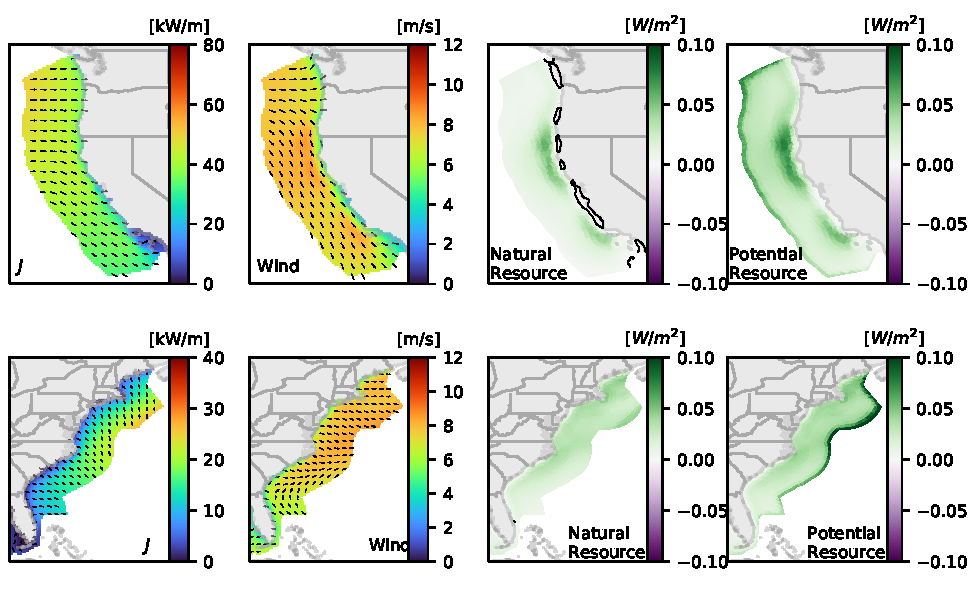
\includegraphics[width=\textwidth]{../fig/Yearly_spatial_seasonal_mag_6.pdf}
  \caption{Maps of average omnidirectional wave power (left), wind (second column), natural resource (third column), and potential resource (roth) for the West Coast (top) and Atlantic Coast (bottom). Black contours show areas of 0 $W/m^{2}$ local or potential resource.}
  \label{fig:maps}
\end{figure}

% \begin{figure}[ht]
%   \centering
%   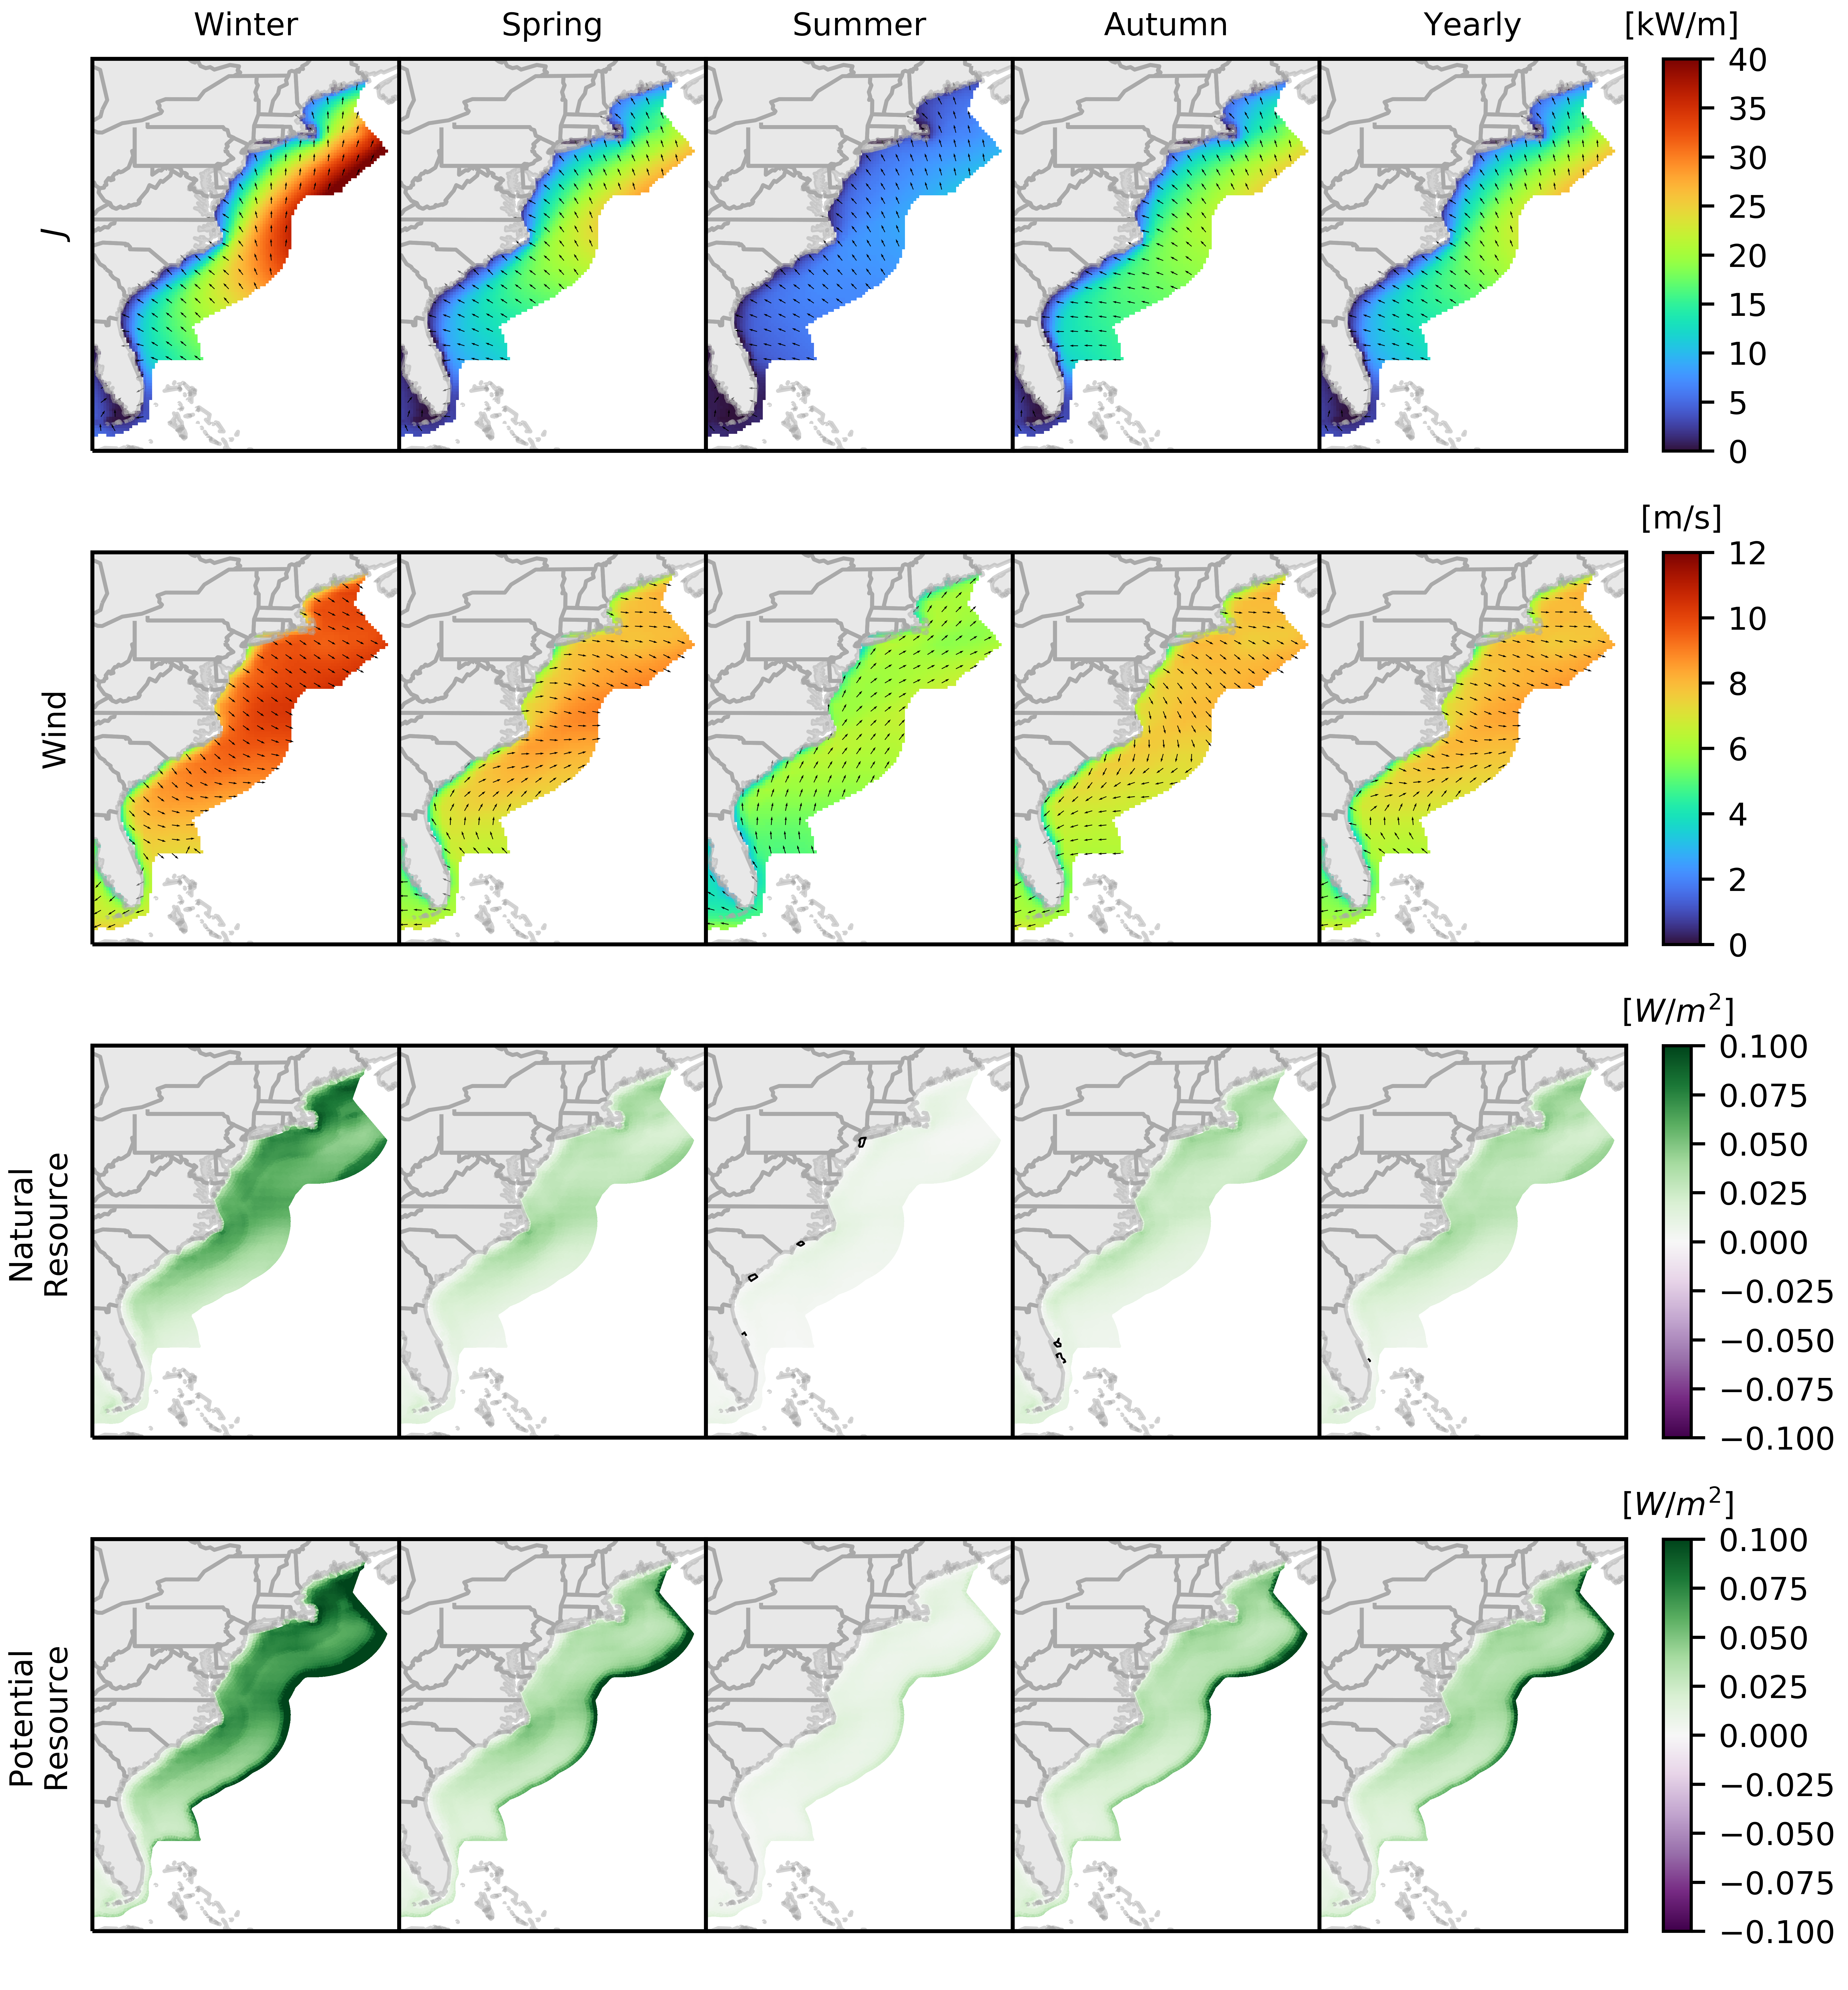
\includegraphics[width=\textwidth]{../fig/at_spatial_seasonal_mag_4.pdf}
%   \caption{Same as \ref{fig:maps-at} for East Coast.}
%   \label{fig:maps-at}
% \end{figure}

\subsection{Annual cycle of wave energy resource}

The annual cycle of the wave energy resource has a remarkably consistent pattern across all U.S. regions (Figure \ref{fig:annual-cycle}). Wave energy is a late-fall and winter dominated resource. The resource peaks in December or January across all regions, and is at a minimum in summer months. The inter-annual variability of the monthly-averaged West Coast resource is small during summer months when the resource is small (Figure \ref{fig:wc-variability}). During energetic winter months, the monthly-averaged resource can vary by more than 50\%, but in general the inter-annual variability is less than 30\% of the month's mean. This suggests that during energetic winter months wave energy projects should be expected to deliver at least their annual mean, with the potential of providing much more than that. However, more detailed analysis is required to demonstrate these characteristics at specific sites and for specific technologies. Other regions have similar variability characteristics (not shown for simplicity).

\begin{figure}[ht]
  \centering
  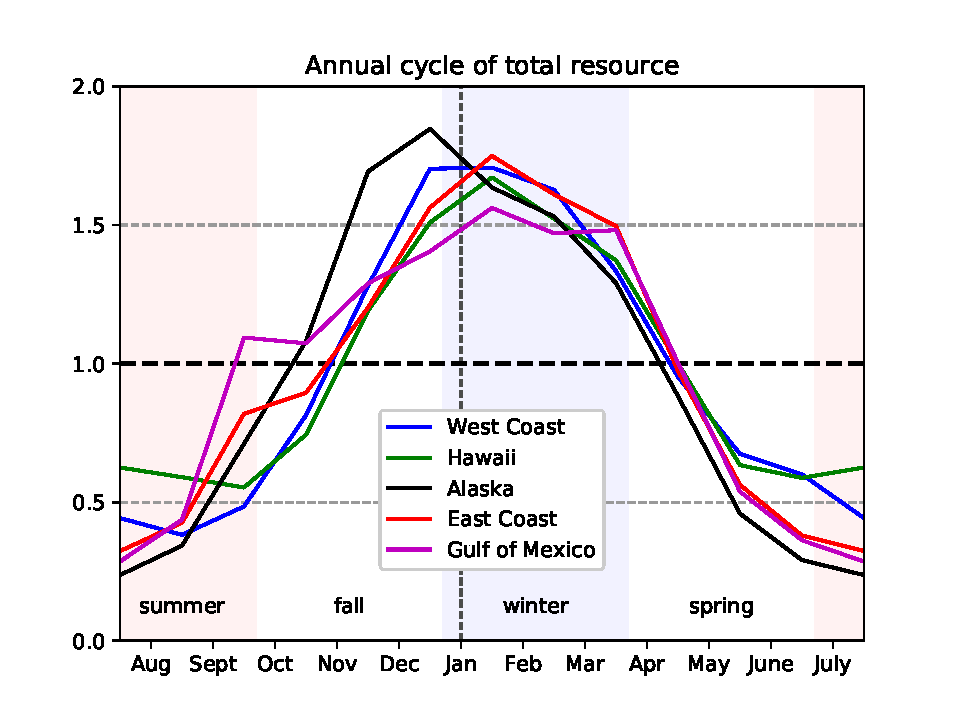
\includegraphics[width=\textwidth]{../fig/AnnualCycle01.pdf}
  \caption[Wave resource annual cycle.]{The annual cycle of the total wave energy resource for several regions, relative to the regional mean.}
  \label{fig:annual-cycle}
\end{figure}


\begin{figure}[ht]
  \centering
  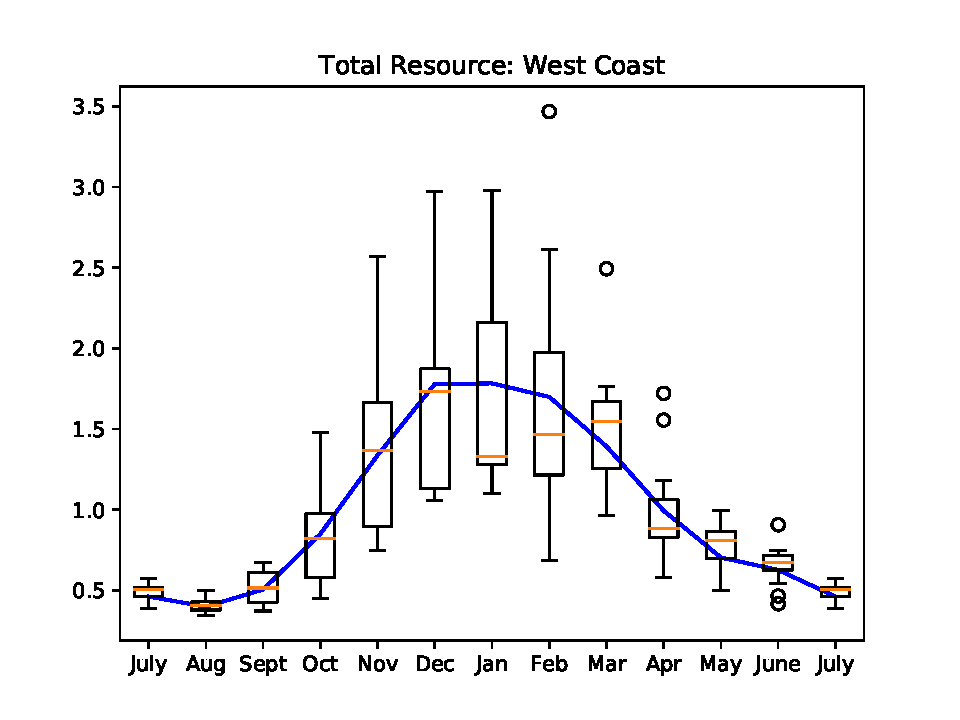
\includegraphics[width=\textwidth]{../fig/AnnualVar01.wc.pdf}
  \caption[West Coast resource variability.]{Annual and inter-annual variability of the West Coast resource. The thick solid line indicates the mean, and the orange lines and boxes indicate the median and quartiles, respectively. The whiskers extend to the last point within 1.5x of the inter-quartile range, and points beyond this are plotted as open-circles.}
  \label{fig:wc-variability}
\end{figure}

\subsection{Wave-period dependence of wave resource}

The US wave energy resource has distinct regional wave-period (frequency) characteristics (Figure \ref{fig:remote-freq}, thick lines). The Atlantic regions (Gulf and East Coast) are dominated by relatively short-period waves compared to the Pacific. The Gulf (including Puerto Rico and U.S.V.I.) resource is particularly high-frequency with a peak at ~6.5 seconds, and 95\% of the energy having a period of less than 12 seconds. The East Coast resource is somewhat lower frequency than the Gulf with a peak at ~10 seconds, and 95\% of the energy less than 15 seconds.

The West Coast resource has a much wider and longer-period distribution, with 90\% of the resource contained between 6.5 and 19 seconds, with a peak at 14 seconds. This is largely because the west coast resource is dominated by long-period swell that has arrived at the U.S. coastline from storms in the distant Pacific (both North and South Pacific). The Hawaiian resource is bi-modal with a peak at 14 seconds and a peak at 9 seconds. This ``double-peak'' is primarily a seasonal effect where waves with period 11-12 seconds are more prevalent in January and February, while waves with period 8-10 seconds arrive in March and April \citep[][]{stopa2013wave}. The Alaskan resource has a spectral peak at 12 seconds, with 90\% of the resource between 6 and 17 seconds.

Finally, we note that including the potential resource (thin lines in Figure \ref{fig:remote-freq}) in the spectral distribution shifts the distribution to higher frequency, and adds a short-period (high-frequency) peak at 2 to 4 seconds compared to the remote only resource (thick lines). This is the influence of the wind input terms, which tend to add energy at high-frequency. The effect is essentially the same when adding the natural local resource (not shown). The low-period (high-frequency) energy contained in the local resource has not typically been of interest to the WEC community, but as interest in niche PBE markets grow - especially those involving small WECs for low power applications - there may be more interest in this portion of the wave energy spectrum.

\begin{figure}[ht]
  \centering
  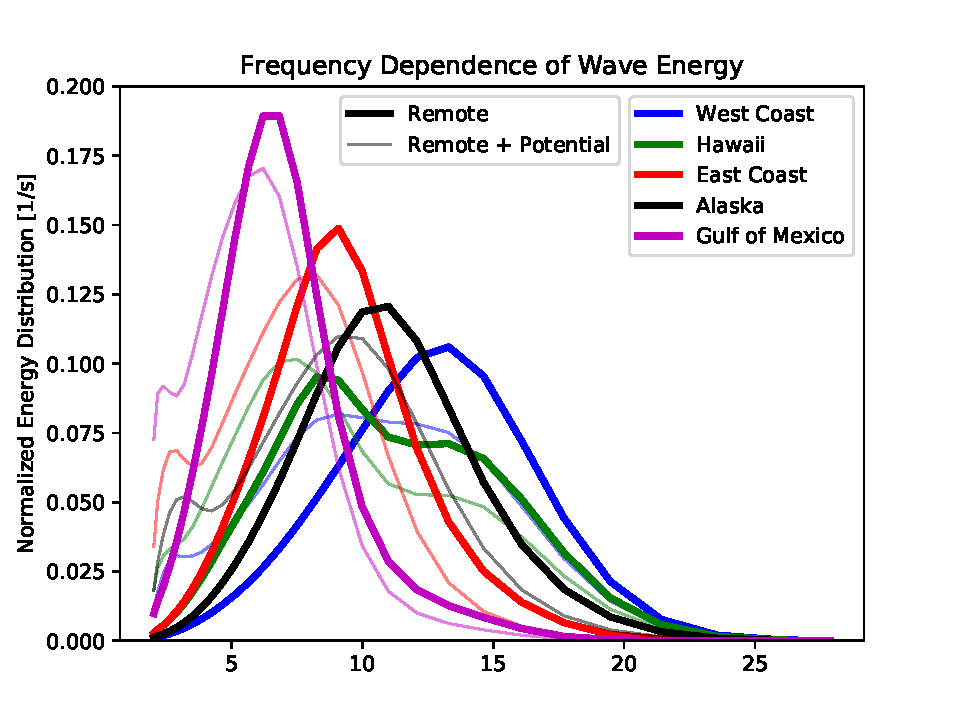
\includegraphics[width=\linewidth]{../fig/TotalResource_Freq02.pdf}
  \caption[Distribution of wave energy vs. wave-period.]{Distribution of wave resource by wave period for each region. Each line represents a spatial average over the entire regional domain. Thick lines indicate the remote resource only, thin lines indicate the sum of the potential and remote resource. Colors are used for each region. Each curve is normalized by its total energy (i.e., the integral of each curve is 1).}
  \label{fig:remote-freq}
\end{figure}

%%% Local Variables:
%%% TeX-master: "wave_res"
%%% End:
